% $Id: template.tex 11 2007-04-03 22:25:53Z jpeltier $
\documentclass{vgtc}                          % final (conference style)

\ifpdf%                                % if we use pdflatex
  \pdfoutput=1\relax                   % create PDFs from pdfLaTeX
  \pdfcompresslevel=9                  % PDF Compression
  \pdfoptionpdfminorversion=7          % create PDF 1.7
  \ExecuteOptions{pdftex}
  \usepackage{graphicx}                % allow us to embed graphics files
  \DeclareGraphicsExtensions{.pdf,.png,.jpg,.jpeg} % for pdflatex we expect .pdf, .png, or .jpg files
\else%                                 % else we use pure latex
  \ExecuteOptions{dvips}
  \usepackage{graphicx}                % allow us to embed graphics files
  \DeclareGraphicsExtensions{.eps}     % for pure latex we expect eps files
\fi%

%% it is recomended to use ``\autoref{sec:bla}'' instead of ``Fig.~\ref{sec:bla}''
\graphicspath{{figures/}{pictures/}{images/}{./}} % where to search for the images

\usepackage{microtype}                 % use micro-typography (slightly more compact, better to read)
\PassOptionsToPackage{warn}{textcomp}  % to address font issues with \textrightarrow
\usepackage{textcomp}                  % use better special symbols
\usepackage{mathptmx}                  % use matching math font
\usepackage{times}                     % we use Times as the main font
\renewcommand*\ttdefault{txtt}         % a nicer typewriter font
\usepackage{tabu}                      % only used for the table example
\usepackage{booktabs}                  % only used for the table 
\usepackage{url}
\usepackage{tabularray}
\usepackage[backend=biber]{biblatex}
\usepackage{cleveref}
\addbibresource{template.bib}

\onlineid{0}
\vgtccategory{Research}

\title{The State-of-Art Platforms and Tools for Immersive Analytical
Applications Development}

\author{Walid Chtioui\thanks{e-mail: walid.chtioui@ensi-uma.tn}\\ %
        \scriptsize University of Passau %
\and Achraf Hebheb\thanks{e-mail: habhabachref@gmail.com}\\ %
     \scriptsize University of Passau}

%% A teaser figure can be included as follows, but is not recommended since
%% the space is now taken up by a full width abstract.
%\teaser{
%  \includegraphics[width=1.5in]{sample.eps}
%  \caption{Lookit! Lookit!}
%}

\abstract{This paper presents an overview of the latest state-of-the-art
platforms and toolkits which can be used to develop immersive analytics (IA)
experiences. Initially, a short overview of Unity3D and Unreal Engine with a
comparison of supported eXtended Reality (XR) features and third party tools
is provided. After that, we present an overview associated with a critique of
what we believe are the major XR development toolkits. For each toolkit we
discuss the set of what we think are important features they provide or lack
such as the support for collaboration, interactions, real-time data and large
datasets. We then present a comparison study between these toolkits with a
particular focus on performance, supported devices, accessibility and
ease-of-use. A set of state-of-the-art tools and techniques, which can be used
to extend aforementioned toolkits, covering collaboration, interaction and
navigation topics are then provided. We have come to the conclusion that,
although IA toolkits have come out of their infancy, we are still yet to see an
IA toolkit that provides a unified workflow allowing for versatile
visualizations, collaboration support, acceptable performance scalability,
real-time data support and support for a plethora of XR and non-XR devices
which has the potential to replicate the wide success of conventional
visualization frameworks such as D3.js.
} % end of abstract

%%%%%%%%%%%%%%%%%%%%%%%%%%%%%%%%%%%%%%%%%%%%%%%%%%%%%%%%%%%%%%%%%%%%%%%%%%%%%%%
%%%%%%%%%%%%%%%%%%%%%%%%%%%%%% START OF THE PAPER %%%%%%%%%%%%%%%%%%%%%%%%%%%%%
%%%%%%%%%%%%%%%%%%%%%%%%%%%%%%%%%%%%%%%%%%%%%%%%%%%%%%%%%%%%%%%%%%%%%%%%%%%%%%%

\begin{document}
\firstsection{Introduction}
\maketitle



\section{Platforms}

Platforms refer to general-purpose frameworks that provide a uniform workflow
allowing developers to create XR applications for a plethora of devices. Since
IA experiences and AR/VR gaming applications share a lot of similarities, game
engines provide excellent support for developing IA experiences. Two game
engines are considered; Unity and Unreal Engine. A particular focus is given
to Unity due to its wide adoptability for XR applications.

\subsection{Unity}
Unity has a wide adoption in the world of XR thanks to its unified workflow
and support for various XR platforms. Unity supports an extensive set of XR
vendor-specific software development kits (hereafter SDK) including: Apple's
ARKit, Google's ARCore, Microsoft's HoloLens and OpenXR. Following the
announcement of Apple's mixed reality (MR) headset Vision Pro in Apple's
Worldwide Developers Conference (WWDC) 2023, Unity was announced to provide
native support for Vision's Pro operating system VisionOS \cite{web:vision_pro_unity}.
Unity also provides a set of XR packages that are built on top of these vendor
plugins to add application-level development tools \cite{unity:xr_packages}.
For instance, AR Foundation is an industry-standard framework that provides
support for various AR features such as: object tracking and plane detection.
Unity also provides XR Interaction Toolkit package which is a high-level,
component-based interaction system. The package also includes XR Device
Simulator which is a simulator that allows user input from conventional input
devices (a keyboard, a mouse or a controller) to drive XR headset and
controllers in the Unity scene view. This may be useful for debugging on a
wide range of XR devices without having to actually try them. Unity also
benefits from open-source external XR packages such as the Mixed Reality
Toolkit for Unity (MRTK)
\footnote{https://github.com/MixedRealityToolkit/MixedRealityToolkit-Unity}
which is designed to further accelerate cross-platform MR development in Unity.
\subsection{Unreal Engine}
\subsection{Comparison}
Figure \ref{table:1} provides a comparison between the previously discussed
platforms in terms of support for vendor-specific SDKs and a set of features.

\begin{table}[ht!]
	\centering

	\begin{tabular}{l c c}
		\toprule
		                              & \multicolumn{2}{c}{\textbf{Platform}}                     \\
		\cmidrule(l){2-3}
		\textbf{SDKs}                 & Unity 2022 LTS                        & Unreal Engine 5.3 \\
		\midrule
		ARCore                        & X                                     & X                 \\
		ARKit                         & X                                     & X                 \\
		Magic Leap                    & X                                     & X                 \\
		Microsof HoloLens             & X                                     & X                 \\
		OpenXR                        & X                                     & X                 \\
		Oculus                        & X                                     & X                 \\
		WebXR                         & X                                     &                   \\
		VisionOS                      & X                                     &                   \\
		\midrule
		\textbf{AR-Specific Features} &                                       &                   \\
		\midrule
		Plane Detection               & X                                     & X                 \\
		Object Occlusion              & X                                     & X                 \\
		Environment Probes            & X                                     & X                 \\
		Face Tracking                 & X                                     & *(ARKit only)     \\
		Object Tracking               & X                                     & X                 \\
		Body Tracking                 & X                                     & ? (not mentioned) \\
		Camera Intrinsics             & X                                     & X                 \\
		Meshing                       & X                                     & ? (not mentioned) \\
		\midrule
		\textbf{XR Features}          &                                       &                   \\
		\midrule
		High-level XR Interactions    & X                                     & ? (not mentioned) \\
		XR Input Simulation           & X                                     & ? (not mentioned) \\
		\midrule
		Vuforia Support               & X                                     &                   \\
		\bottomrule
	\end{tabular}


	\medskip

	\caption{Per-platform supported SDKs, AR features and 3rd party tools.}
	\label{table:1}
\end{table}

\section{Toolkits and Frameworks}

The term toolkit refers to development environments that are tailor-made for
IA experience development purposes. They provide, among other things,
high-level tools for authoring visualizations, built-in interactions and
support for multiple major XR devices.

\subsection{DXR Toolkit}

Sicat et al. proposed DXR \cite{dxr_toolkit}; an IA toolkit built on top of Unity
that allows fast prototyping and iteration for non-experienced users; i.e.
users with no or little programming knowledge in XR and Unity.
Alongside the data input, DXR takes a specification file written in JavaScript
Object Notation (hereafter JSON) from which visualisations are created.
The specification file is described in Vega-Lite declarative grammar \cite{vega_lite}
(only what should be achieved has to be provided, not how) making it suitable
for users with no programming experience to rapidly realise immersive
visualisations. This configuration file can be edited in a separate text editor or through
the use of a GUI with pre-configured set of parameters. DXR also provides
built-in specification templates for common visualisations such as: Scatter
plots and bar charts. This further extends the scope of users to include
those without any technical experience. Although the authors claim that DXR
provides suitable flexibility, the scope of that flexibility seems to be
limited to providing, among other things, custom graphical markers, custom
visualization channels - i.e. a visualisation parameter affected by a
data dimension - and other visualisation-type specific properties. That limits users to a
templated and common set of visualisations such as scatter plots, bar charts
and radial bars. There is also no mention of real-time data support thus
limiting the use case of DXR to offline data only.

\smallskip

\noindent As the authors have explicitly mentioned, DXR is meant for
prototyping and exploring designs, it is not designed to handle visualisations
of large datasets. On HoloLens, for datasets with more than approximately
a thousand item, suboptimal - less that 60 frames per second (hereafter FPS) -
performance has been observed. Nonetheless, the authors argue that DXR can still
be useful for quickly and cheaply prototyping large dataset designs before
moving to specialized, optimized and detailed implementations.

\subsection{IATK Toolkit}
Maxime et al. introduced IATK \cite{iatk_toolkit}; an open-source
\footnote{https://github.com/MaximeCordeil/IATK} software
package for Unity that provides both a high-level Unity-editor-integrated GUI
for simple authoring and a low-level C-sharp and JavaScript API for
fine-grained authoring and extending the visualizations.

\smallskip

\noindent To some degree of similarity to DXR, IATK relies on a high-level
declarative grammar of graphics by providing a composable grammar of
visualization primitives alongside a high-level interface for rapid prototyping
and iterations. What sets IATK apart, is that it was designed with scalability
in mind, a focus on large and complex multidimensional datasets and a focus on
user interactions. The toolkit's authors claim that it can render millions of
items thanks to its use of efficient GPU shader code. Also, contrary to DXR,
IATK does not support declarative configurations, instead it relies on a Unity
editor GUI or C-sharp API code that make use of a composable grammar to author
visualizations.

\smallskip

\noindent Unlike DXR and other toolkits built on top of Unity, IATK does not
render the datapoints (here we do not mean point as in a geometrical point but
as a representation of a data entry) as Unity game objects and use
expensive-to-update-at-large-scale object attributes as visualization channels.
Instead, all the datapoints are visualized within one game object where each
data point is encoded into a unique vertex by mapping data attributes,
such as position, color and size, into vertex components such as vertex UV
coordinates, vertex normal vector and vertex color. This way, actual datapoint
geometries are created on the GPU resulting in a potentially more
efficient rendering process. This however greatly limits the customizability
of datapoint marks and the choice of visualization channels especially for
novice users.

\smallskip

\noindent According to the authors' performance statistics, on VR less than
90 FPS is observed at two million datapoints and on AR less than 60 FPS is
observed at just a thousand datapoints. However, one can subjectively claim
that the performance on AR HoloLens headset remains acceptable up-to ten
thousand datapoints at which 41 FPS is achieved. Although the authors provided
FPS statistics for Oculus CV1, Meta2 and HoloLens devices, no performance
statistics were provided for the alternative game-object-based datapoint
approach to provide a performance reference point.

\begin{figure}[tb]
	\centering
	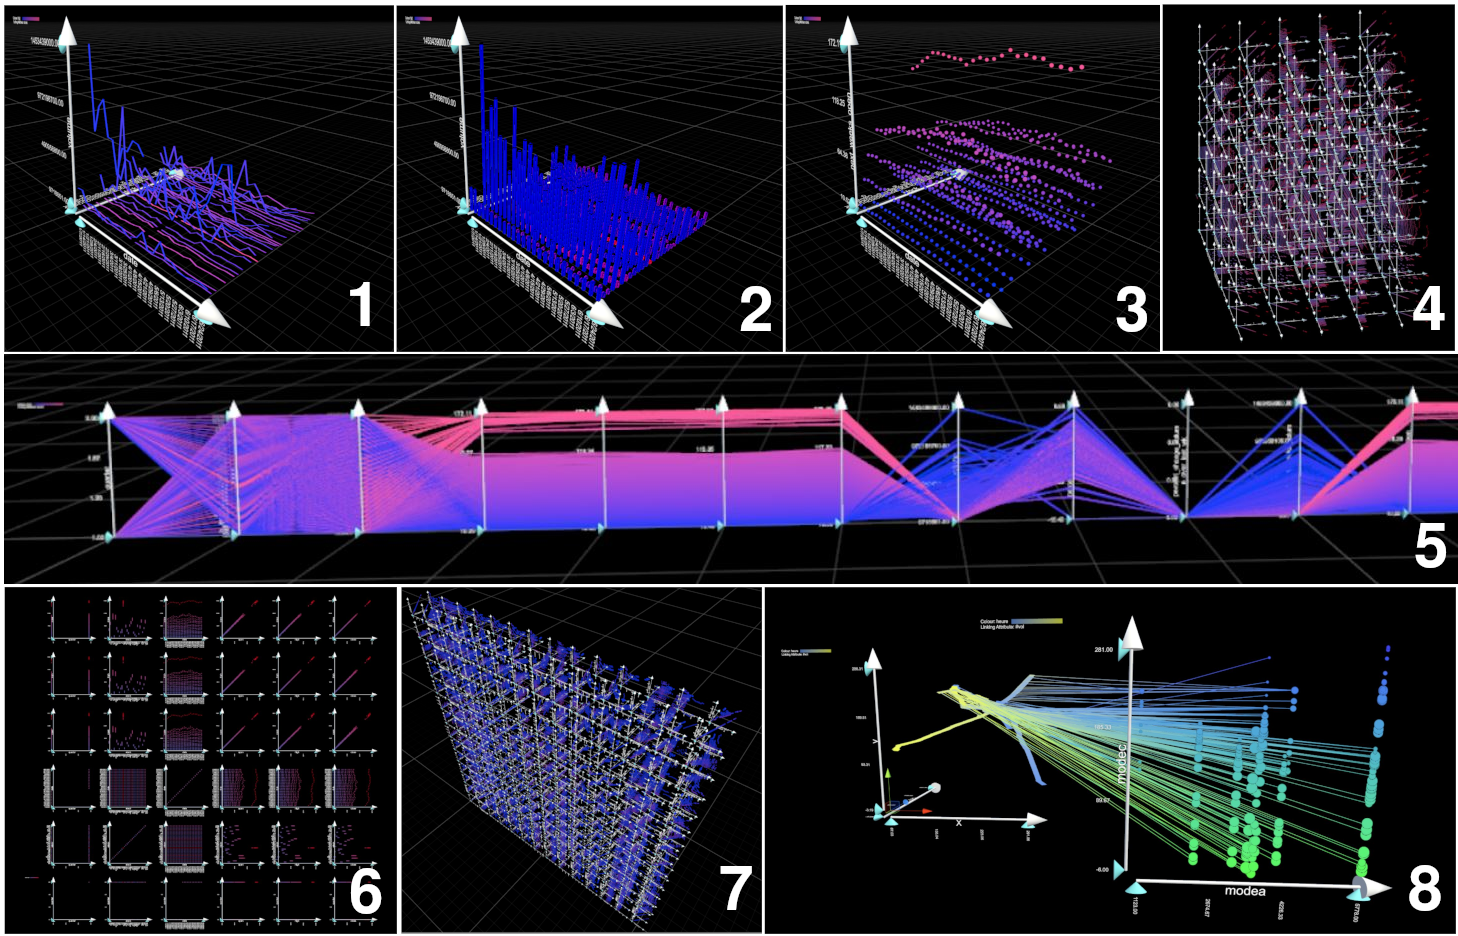
\includegraphics[width=\columnwidth]{iatk}
	\caption[Caption for IATK]{IATK supported visualization types. (1) 3D
		connected dots. (2) 3D bar chart. (3) 3D Scatterplot. (4, 7) 3D
		Scatterplot matrix. (5) Parallel Coordinates Plots. (6) 2D Scatterplot
		matrix. (8) Linked visualizations. The images are from \textsuperscript{1}
		and are in the public domain.}
	\label{fig:iatk_visualizations}
\end{figure}


\smallskip

\noindent IATK integrates an interactive visualization model within its
visualization components that allows a set of interactions including filtering,
brushing and linking (\cref{fig:iatk_visualizations} (8)), details on demand,
animated transitions and attribute-based animations. These interactions are
implemented in the vertex Shader part of the rendering pipeline which leverages
the high parallelism nature of the GPU(s) making them particularly responsive
and efficient at handling large datasets.

\smallskip

\noindent IATK's high-level GUI provides just a small set of built-in visualization
types such as a 3D\textbackslash2D Scatterplot (\cref{fig:iatk_visualizations}
(3)), a parallel coordinates plot (\cref{fig:iatk_visualizations} (5)) or a
3D\textbackslash2D Scatterplot matrix (\cref{fig:iatk_visualizations} (4, 6, 7)).
It also only provides a small set of datapoint geometries. To extend these,
one has to use the provided low-level API which might limit expressiveness for
non-experienced users.

\smallskip

\noindent The authors did not mention any support for neither real-time data
visualization nor local or remote collaboration. It is also worth mentioning
that for VR, only Scatterplot visualization type is supported. This greatly
limits the expressiveness for VR users.

\subsection{VRIA Toolkit}
Peter et al. introduce VRIA \cite{vria_framework}; a free and open-source \footnote{https://github.com/vriajs}
framework for building IA experiences in VR. Unlike the aforementioned
toolkits, VRIA is not built as an add-on on top of a game engine. Instead, it is
built upon open-standard Web-based frameworks such as WebVR, A-Frame, React and
D3.js. All of which are mature, open-source and widely used Web-based
frameworks and libraries. This allows VRIA applications to be accessible by a
plethora of VR and non-VR devices.

\smallskip

\noindent The toolkit is designed to be accessible to novices and experts
alike. Similar to DXR, VRIA makes use of a declarative grammar similar to
Vega-Lite \cite{vega_lite} which allows users to create custom visualizations based on a configuration
file. However, this visualization configuration file is only required for
basic functionalities. For extra custom functionalities such as a custom set of
visualization channels, interactions, graphical marks or visualization types,
more experienced users are advised to use the provided low-level API.
VRIA provides The VRIA Builder; a Web application intended for beginners that
integrates a GUI and a 3D scene view to rapidly prototype visualization designs
with instant feedback without having to leave the browser. It is worth
mentioning that, unlike DXR, this customization GUI is not part of the VR scene
and cannot be viewed withing the VR headset. Only the scene view can be
experienced immersively. However, the authors mentioned their willingness to
add \textit{in-situ} GUI so that users can build and prototype visualizations
iteratively without having to remove the headset and switch back to desktop
screen.

\smallskip

\noindent Thanks to its composable structure, the toolkit can be integrated into
other existing 2D or immersive visualization applications. For instance,
VRIA's visualizations can be overlaid on top of another A-Frame scene.
VRIA has support for collaborative immersive analytics through either the
high-level networking abstraction layer provided by the open-source Networked
A-Frame component or by using the provided API with lower-level networking
libraries.

\smallskip

\noindent In terms of data input, the toolkit only supports tabular data in the form of
JSON or CSV thus real-time data visualization is not supported. The authors
expressed their willingness to add support for other forms of data models such as
geospatial GeoJSON, network and relational models.

\smallskip

\noindent The authors stated that VRIA offers the option to integrate D3.js
visualization within its IA experiences. D3.js is web-base JavaScript
visualization library that provides a low-level approach to author graphics and
powerful mechanisms to transform and manipulate data. Since D3.js is widely
adopted, integrating it within VRIA allows for easier usability and quicker
authoring of 2D visualizations. However, there was not a description of
which D3.js functionalities and visualizations are integrable nor any guidance
on how to integrate it within the VRIA framework.

\smallskip

\noindent More experienced users seeking for a more custom experience are
forced to deal with two separate tools to author custom visualizations;
the visualization configuration file specified in a declarative language and
the API specified in JavaScript. We believe that it would be easier for the end users if VRIA
provided more customizability through the visualization configuration file instead of just
providing very basic functionalities.
Although it is understandable that A-Frame simplifies the process of creating
VR experiences on the web relative to the lower level Three.js library, we
question its necessity. A-Frames' functionalities could be directly implemented
in Three.js thus reducing and simplifying the VRIA stack. The authors stated
their intention to work at the Three.js level directly without the usage of any further
abstraction libraries.

\smallskip

\noindent Whenever 3D graphics are mentioned in the context of web browsers,
performance implementations are one of the most worrying aspects. This is
especially true for Web-based VR applications where two images have to be
rendered each frame preferably at 90 FPS to avoid motion sickness. VRIA's
authors provided visualization benchmarks on a desktop monitor, a desktop
Oculus Rift CV1 and a smartphone. A scatter-plot visualization type was used
with sphere graphical marks. The exact set of visualization channels used
was not mentioned neither were attributes of the input data. On the desktop
monitor and Oculus Lift HMD, performance drops significantly after one
thousand data points. On smartphone performance starts dropping at one hundred
data points. This proves that VRIA is not suitable for large dataset
visualizations. The authors claim that the performance observed for the HMD
is similar to that of IATK for the HoloLens device. But the HoloLens uses
its own, much less powerful, hardware while VRIA performance benchmark used
the Oculus Lift CV1 VR HMD which relies on a separate desktop for expensive
rendering operations. We therefore question such comparisons of performance
benchmarks. This is later Web-based XR solutions do not compete,
in terms of performance, with game-engine based solutions.

\smallskip

\noindent VRIA only supports Cartesian plots but the authors expressed their
willingness to add support for other coordinate systems including geographical
and spherical coordinates.
Moreover, although the authors showcased the ease of integrating VRIA with
AR.js to target AR experiences, the absence of an out-of-box support for VRIA
still limits AR accessibility only to experienced users.

\subsection{RagRug Toolkit}

\begin{figure}[tb]
	\centering
	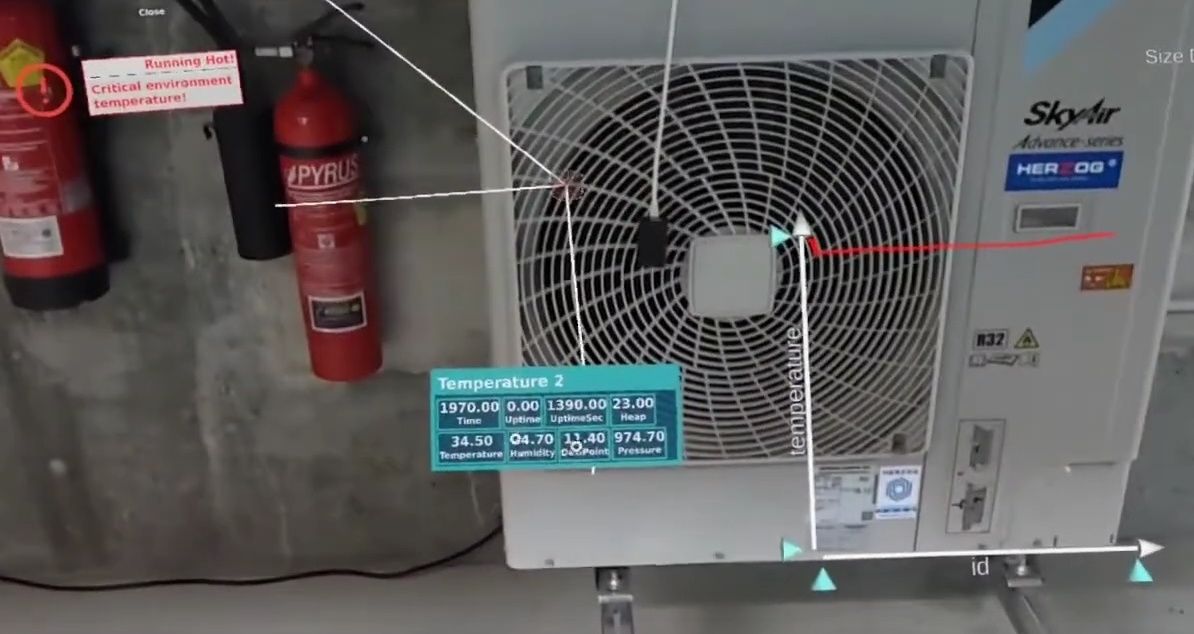
\includegraphics[width=\columnwidth]{ragrug_example}
	\caption[Caption for RagRug]{Example of situated analytics using RagRug
		toolkit. Multiple visualizations are shown and are fed real-time
		temperature data from nearby IOT sensor devices.
		Image from \textsuperscript{4} and is in the public domain. }
	\label{fig:ragrug_example}
\end{figure}

Philipp et al. presented RagRug \cite{ragrug_toolkit}; An open-source
\footnote{https://github.com/philfleck/ragrug} toolkit built on top of IATK
for \textit{situated analytics}, i.e., real-time data-fed interactive immersive
visualizations connected to a meaningful physical object in close proximity to
the user (hereafter we refer to such an object as a \textit{referent}).
For instance, a facility manager equipped with an AR HMD, when in proximity to
an air conditioner with multiple Internet-of-Things (IoT)
sensor devices monitoring temperature and other parameters, multiple real-time
visualizations pop up (\cref{fig:ragrug_example}). Since it only targets
situated-analytics usecases, RagRug is an AR-only toolkit.
A major requirement for IA toolkits is to provide support for a wide variety of
input and output modalities spanning VR/AR and potentially conventional 2D
screen displays. RagRug aims, on top of that, to achieve a broad coverage of
IoT devices.

\smallskip

\noindent The core design goals and features of RagRug are:
\begin{itemize}
	\item \textbf{Providing 3D Visual Encoding Capabilities} -
	      RagRug should provide 3D \textit{visual encoding} capabilities, i.e.,
	      ways of mapping data dimensions into 3D visual structures. These
	      capabilities are inherited from IATK and the visual representations
	      are the same.
	\item \textbf{Making Visualizations Context Aware} -
	      The toolkit should provide visualizations that are context-aware with
	      regards to changes in the real world. This reduces the need to
	      explicitly specify every minute detail while the user is emerged in
	      a physical task. For instance, If a referent is moved, the attached
	      visualization should move along with it or if the lighting conditions
	      change then visualization color should adapt to such new condition
	      or if the user performs an invalid action, a notification is
	      adequately shown. RagRug makes use of IoT devices for collecting data
	      about the environment and a cloud server for, among other things, the
	      IoT application logic and depositing data in a database backend
	      so that the client can query it dynamically.
	\item \textbf{Supporting a Comprehensive Physical-Virtual Model} -
	      Information about the characteristics of referents such as location,
	      shape or identity should not be hard-coded and should instead be
	      queried from a suitable database. That way the client obtains
	      relevant data dynamically. This is important for correctly linking
	      visualizations to referents.
	\item \textbf{Making the Visualization Pipeline Reactive} -
	      The pipeline should be re-evaluated after every external change. For
	      instance, when new data comes, visualizations should be updated or
	      when a device is turned off, marks in a visualizations should be
	      changed to reflect that. IATK lacks support for neither real-time
	      data (since it expects a static dataset input) nor for receiving
	      events from external sources. To address this, RagRug relies on an
	      extension on top of IATK to update data points on network events
	      locally and externally.
	\item \textbf{Supporting Situated Authoring of Visualizations} -
	      Since testing situated analytics requires physical interactions with
	      referents, not allowing for situated authoring may result in a
	      cumbersome development experience. The authors propose runtime
	      interpretation of application logic which allows designers to modify
	      every aspect of the system without having to shut it down. To address
	      the lack of in-situ authoring from IATK, The authors make use of
	      PowerUI \footnote{https://github.com/Kulestar/powerui}, an
	      open-source JavaScript extension for Unity that allows for UI
	      authoring using CSS, HTML and JavaScript.
\end{itemize}

\begin{figure}[tb]
	\centering
	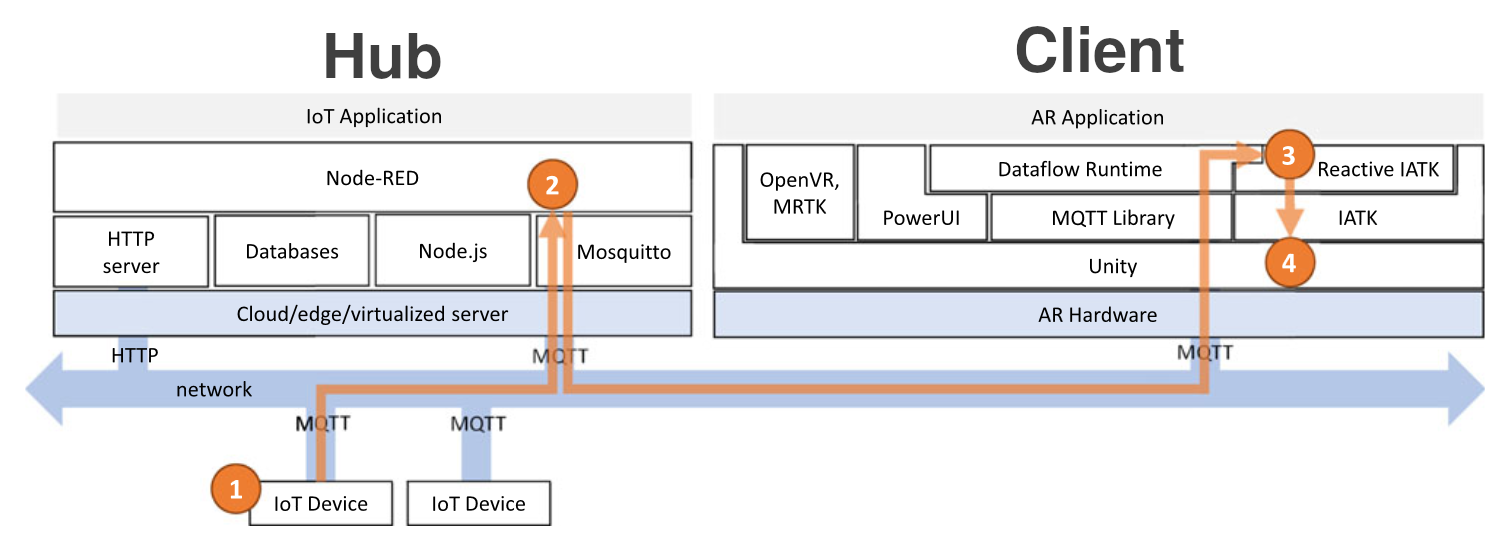
\includegraphics[width=\columnwidth]{ragrug_stack}
	\caption[Caption for RagRug]{RagRug stack. (1) Data is acquired from IoT
		sensors using MQTT. (2) Data filtering. (3) Real-time data is sent to
		IATK as a response to a query. (4) Visualizations are
		rendered/updated in Unity.}
	\label{fig:ragrug_stack}
\end{figure}

\medskip

\noindent RagRug consists of two standalone platforms, one for experiencing
immersive analytics visualizations and interacting with them (hereafter we
refer to this as the \textit{client}) and one for IoT applications and
databases (hereafter we refer to it as the \textit{hub}). As illustrated
in (\cref{fig:ragrug_stack}) the two platforms make use of the widely adopted
and lightweight MQTT \footnote{https://mqtt.org/} protocol to communicate
data and events.

\medskip

\noindent The authors showcased five application examples with a varied level of
sophistication.

We find the use of PowerUI extension questionable, since it has been deprecated
from the Unity Asset store and the open-source GitHub repository has been
inactive for more than five years.

\subsection{Comparison}

\section{Prototypes}

While tools refer to systems that aim to allow developers to create IA
experiences, prototypes are applications that target end-users by providing IA
experiences attempting to solve particular IA-related and/or domain-specific
problems. Through the feedback of end-users, prototypes may provide interesting
insights on how IA tools should address particular challenges.


\subsection{Fiesta}

\noindent Benjamin et al. built FIESTA \cite{fiesta_prototype}; an open-source
\footnote{https://github.com/benjaminchlee/FIESTA} team-based analysis
prototype that allows users to create, manipulate and share data visualizations
in an unconstrained and physically co-located VR-only environment. The authors
state that the main objective behind developing FIESTA is to study how groups
collaboratively explore data in a free-roaming VR environment.

\medskip

\begin{figure}[tb]
	\centering
	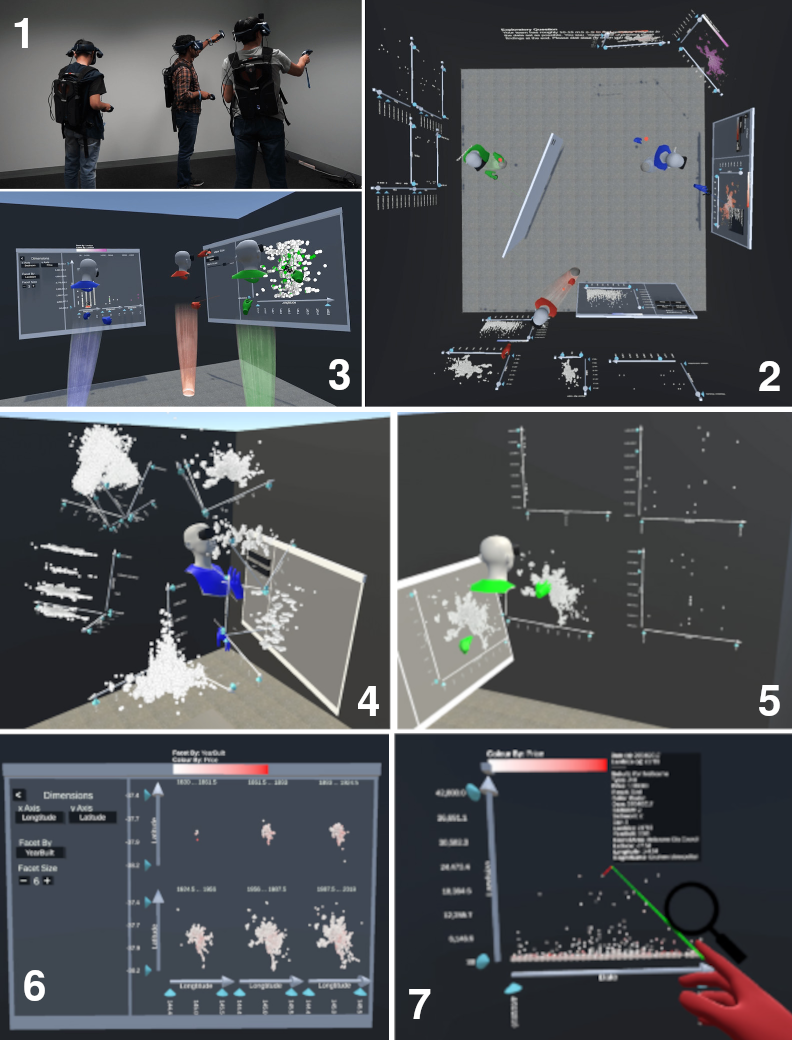
\includegraphics[width=\columnwidth]{fiesta}
	\caption{(1) Real view of participants using the FIESTA system. (2)
		Top-down view of a virtual scene in which three participants are
		conducting visual analytics tasks. (3) A virtual view from the perspective of an
		observer. (4) Egocentric layout. (5) Planar layout. (6) Authoring panel
		with a faceted scatterplot on its right interface. (7) Details on
		demand to easily inspect data records. All images are taken from
		\cite{fiesta_prototype}.}
	\label{fig:fiesta}
\end{figure}

\noindent FIESTA is built on top of IATK. The authors justify the usage of IATK
for performance reasons since multiple users can each produce multiple
visualizations. A 16m\textsuperscript{2} (4m x 4m) room is used to conduct the
study. Each user is equipped with a VR headset and a backpack containing a
laptop to which the headset is connected (\cref{fig:fiesta} (1)). To track the
headsets' positions, four trackers are positioned in the room; one in each
corner. An additional desktop PC manages the users' laptops using the Unity
networking engine Photon. Although the study focuses on physically co-located
IA environment, the authors state that the research prototype also supports
remote collaboration.

\medskip

\noindent The core design goals and features of FIESTA are:
\begin{itemize}
	\item \textbf{Baseline Visualizations} - The prototype provides three types
	      of 2D and 3D visualizations: scatterplots, faceted scatterplots
	      (\cref{fig:fiesta} (6)) and line charts.
	\item \textbf{Baseline Interactions} - FIESTA relies on standard
	      interfacing techniques across desktop and VR. It provides grasping
	      techniques for interacting with UI elements at close range and ranged
	      pointing techniques using a laser pointer for long range
	      (\cref{fig:fiesta} (7)).
	\item \textbf{Baseline Authoring} - Each user is provided with a movable
	      panel to author visualizations (\cref{fig:fiesta} (2, 3, 4, 5, 6)).
	      The panel is split into two sections: on the left, a GUI is provided
	      to map data dimensions to visualization channels, choosing the
	      faceting dimension and adjusting the number of facets; the right
	      panel is used to show produced visualizations.
	\item \textbf{Tearing out Visualizations} - Visualizations can be cloned
	      from the panel by grasping and pulling them away. These cloned
	      visualizations can then be placed independently in the 3D space
	      (\cref{fig:fiesta} (2, 4, 5)). Resizing and rescaling operations are
	      supported through grasping interactions on widgets placed along
	      visualization object's axis. Visualizations can also be brought back
	      into the panel for further editing or be destroyed through a
	      throwing-towards-ground interaction.
	\item \textbf{Linked Brushing} - Private and shared brushes are provided
	      for each user. The private brush allows for selections that are only
	      visible to the user while the shared brush allows for selections
	      which are visible to all users. Brushing is linked across multiple
	      visualizations through color channel, i.e. contrary to other tools
	      where lines are used to visualize linked datapoints.
	\item \textbf{Pointer and Details on Demand} - A pointer is provided and is
	      activated through controller's trigger. Details-on-demand tool of the
	      nearest datapoint is enabled through a touchpad input
	      (\cref{fig:fiesta} (7)). The pointer can also be used to interact
	      with the panel's interface through point-and-click interaction for
	      buttons or point-and-drag interaction for sliders and pickers.
	\item \textbf{Free Roaming Shared Environment} - To emulate a physically
	      co-located collaborative environment, Each user is represented by a
	      uniquely colored avatar and a floating nameplate
	      (\cref{fig:fiesta} (3)). The same unique color of the user's avatar
	      is used for coloring shared brush selection. There is no ownership
	      system in FIESTA; everything is seen and interactive by all users
	      except the private brush tool.
	\item \textbf{Room and Surface Affordances} - To explore how users
	      naturally use surface-based functionalities in collaborative IA
	      environments to solve visual analytics tasks, a four-wall room with
	      a square tabletop in the center is used. The virtual walls act as a
	      boundary to prevent users from hitting the actual room walls.
	      Releasing visualizations close to the virtual surface of the table
	      top make them rest on top of it.
\end{itemize}

\medskip

\noindent A total of 30 participants were recruited for the study with all but
one having a background in computer science. The participants managed to
perform visual analytics tasks and remained engaged with these tasks for 45
minutes on average. This proves that collaborative visual analysis is possible
in VR. Participants made use of 3D visualizations although their use was not
emphasized. They came up with interesting ways to view them such as: scaling a
3D visualization to room scale and standing in the middle of it; laying 3D
visualizations around them in an egocentric layout (\cref{fig:fiesta} (4)) and
looking at them from an axis-aligned viewpoint. With 2D visualizations,
participants preferred placing them in a grid-like layout on the walls. This
made them more presentable to others at all times contrary to 3D visualizations
where users struggled to take the perspective of observers into consideration
when viewing them. Therefore, IA tools should explore methods to facilitate the
presentation of 3D visualizations to other users. Another interesting
observation is that 3D visualizations heavily influenced the way 2D
visualizations are organized. For instance, in the presence of 3D
visualizations, these 2D visualizations were placed in an egocentric layout.
These observations demonstrate the importance of a consistent UI design that
supports both 2D and 3D visualizations. The study findings may also justify
the need to provide different placement tools for 2D and 3D visualizations.
Furthermore, although the usage of surfaces is completely optional in FIESTA,
participants made use of the walls to neatly place their 2D visualizations.
However, they saw no benefit in using the central table top for visualization
placements. This demonstrates that users are influenced by environment
configuration only if there is a tangible benefit to its usage. The majority
of users mixed between individually and collaboratively working although both
modes were optional in FIESTA. This proves that providing support for both
working modes is invaluable. The study also showed that participants did not
interact with objects that, except in cases where such interactions were
expected, did not belong to them. However, the reason behind that could be
avoiding physical collisions with other users. Therefore a study with remotely
co-located environment is needed to further study these behaviours.

\medskip

\noindent Although the usage of surfaces is optional in FIESTA, they were
inherently predefined - the users did not have the option to arrange such
surfaces. A similar system in which they have to ability to define their own
surfaces may further expand these findings. Furthermore, FIESTA is a VR-only
prototype therefore these findings may not be applicable to IA experiences
where AR is used.


\subsection{Uplift}
Barrett et al. proposed Uplift \cite{uplift_prototype}; an in-place
collaborative visual analytics prototype targeting users with diverse
expertise in the domain of microgrids. Uplift is designed for casual visual
analysis use-cases; i.e. to be used to easily identify, in a relatively short
time, key patterns in complex visualized data. The requirements for the
prototype were initially provided and subsequently modified, through multiple
feedback sessions, by a wide range of stakeholders including microgrid project
and energy systems experts.

\begin{figure}[tb]
	\centering
	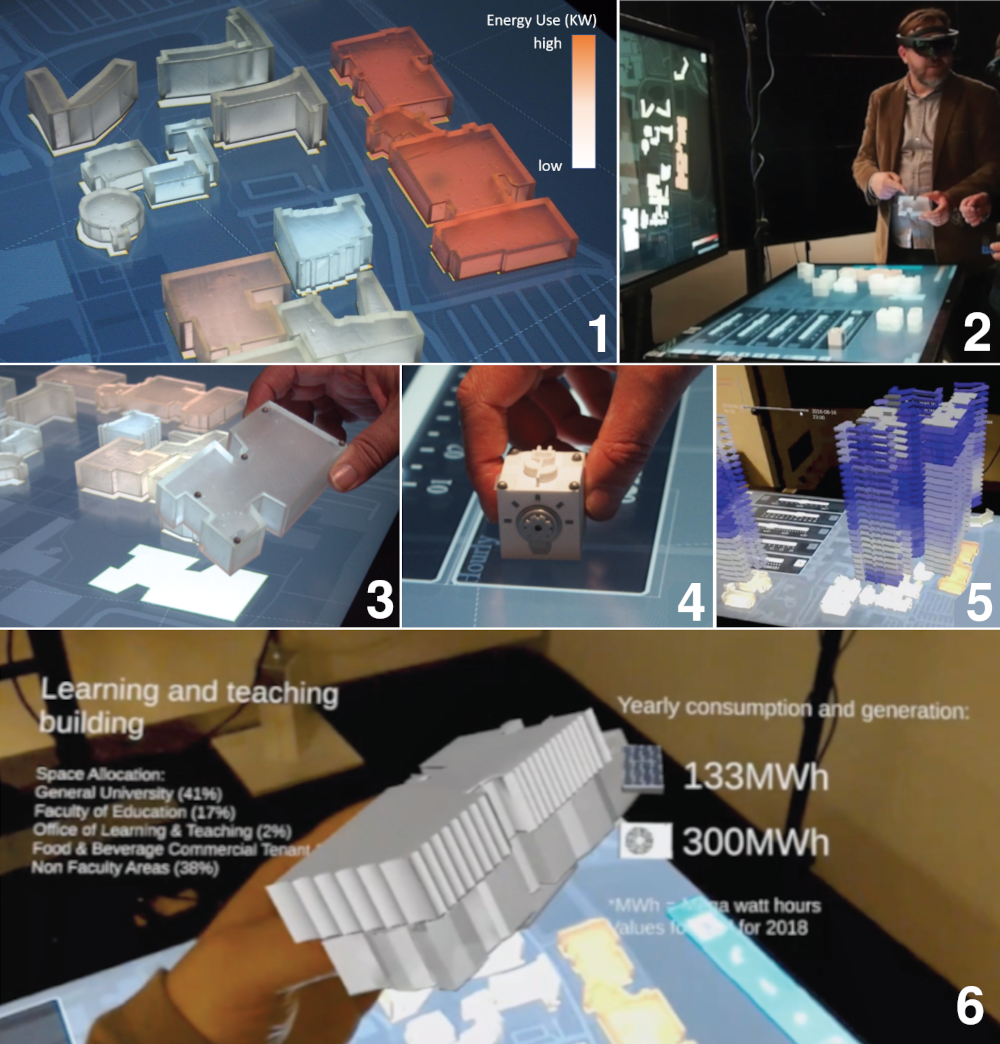
\includegraphics[width=\columnwidth]{uplift}
	\caption[Caption for Uplift]{A showcase of Uplift prototype. (1)
		Translucent scaled-down models of campus buildings placed on top of the
		colored tabletop to reflect energy consumption. (2) Users gathering
		around the central tabletop supported with a large 2D display. (3)
		A user picking up a scaled-down building model of the campus. (4)
		A user interacting with a tangible widget affecting a slider which
		in turn affects time granularity and therefore the number of slices
		in (5). (5) AR for visualizing data above and around the central
		tabletop, in particular hourly energy consumption is visualized as 2D
		slices laid over buildings. (6) A picked-up campus scaled-down building
		model overlaid with relevant data by AR.
		Images from \cite{uplift_prototype}.}
	\label{fig:uplift}
\end{figure}

\medskip

\noindent The main design goals of Uplif that were identified through multiple
stakeholders feedback sessions are:
\begin{itemize}
	\item \textbf{Walk Up and Use}: The system should be inviting, intriguing and
	      compelling.
	\item \textbf{Low Technical Barrier to Entry}: Easily usable by users with a wide
	      degree of technical knowledge.
	\item \textbf{Supports Multiple Participants}: Provide flexible collaboration
	      support to small and large groups alike.
	\item \textbf{Supports Analytical Sprints}: Provide support for short analytical
	      activities.
\end{itemize}

\medskip

\noindent Uplift relies more than just AR headsets to bring casual
collaborative visual analytics to a multitude of microgrid stakeholders.
A tabletop display showing a geographical map of the campus grid is used as a
central platform where users are supposed to gather around and interact with
widgets placed on top of it (\cref{fig:uplift} (2)). Uplift also makes use of
tangible widgets which are physical and interactive elements that control
visualization parameters (for instance by affecting sliders) (\cref{fig:uplift}
(4)). The prototype also relies on scaled-down physical models of buildings
that are translucent which allows the color of the surface on which they are
placed to be used as an appealing visualization channel
(\cref{fig:uplift} (1)). If these models are picked up, AR will overlay
relevant data about them (\cref{fig:uplift} (6)). AR is used to display
multiple 3D data types on top of the tabletop and 2D graphs alongside legends
around it (\cref{fig:uplift} (5)). On top of these, Uplift uses a large display
to either replicate the content of the tabletop or show additional
visualizations (\cref{fig:uplift} (2)).

\medskip

\noindent Through the feedback of 16 participants who tried the prototype,
Uplift was proven to be potentially useful for microgrid-related data
analytics.

\medskip

\noindent Although Uplift was designed for microgrid-related systems,
the authors claim that its applicability domain can be extended to include
other fields that rely on analysis of complex spatial data for sense-making
such as the construction industry. However, the use of a wide range of technologies
and gadgets makes Uplift a specialized solution that we believe is not yet
ready for wide deployment. For instance, on top of using Vuforia for tabletop
tracking, Uplift uses the motion capture Vicon system
\footnote{https://www.vicon.com/} with a proprietary tracking software and four
cameras to track the tangible widgets and the buildings. However,
since no proof was provided for the usefulness of overlaying information when
a building model is picked, we question the usage of object tracking for this
purpose. This is particularly true if such feature requires the addition of
expensive gadgets and proprietary software. For instance, model position is
already embedded in the tabletop map visualization and that can be used by AR
to overlay visualizations above without the need of object tracking. We also
argue that the use of tangible widgets to control visualization parameters does
not justify the usage of additional gadgets and software required to track
them.

\medskip

\noindent Uplift expects a static data input therefore, although the topic of
real-time monitoring of the microgrid was seen as beneficial for operators by
expert stakeholders, the tool does not support real-time immersive analytics.

\section{Collaboration Tools and Techniques}

\section{Interaction Tools and Techniques}

Interaction is an important component of information visualization. It has even
been argued that it provides a way to overcome the limits of representation and
augment a user's cognition \cite{interaction_infovis}.

\section{Navigation Tools and Techniques}

\section{Transition and Animation Tools and Techniques}

TODO: add introduction with suitable references for importance of animations
and cross-virtuality transitions.
\subsection{HybridAxes Tool}
Mohammad et al. introduced HybridAxes \cite{hybridaxes_tool}; an extension of
IATK toolkit that allows for a smooth interoperability between 2D desktop
visualizations and immersive reality experiences (\cref{fig:hybridaxes}).

\medskip

\begin{figure}[tb]
	\centering
	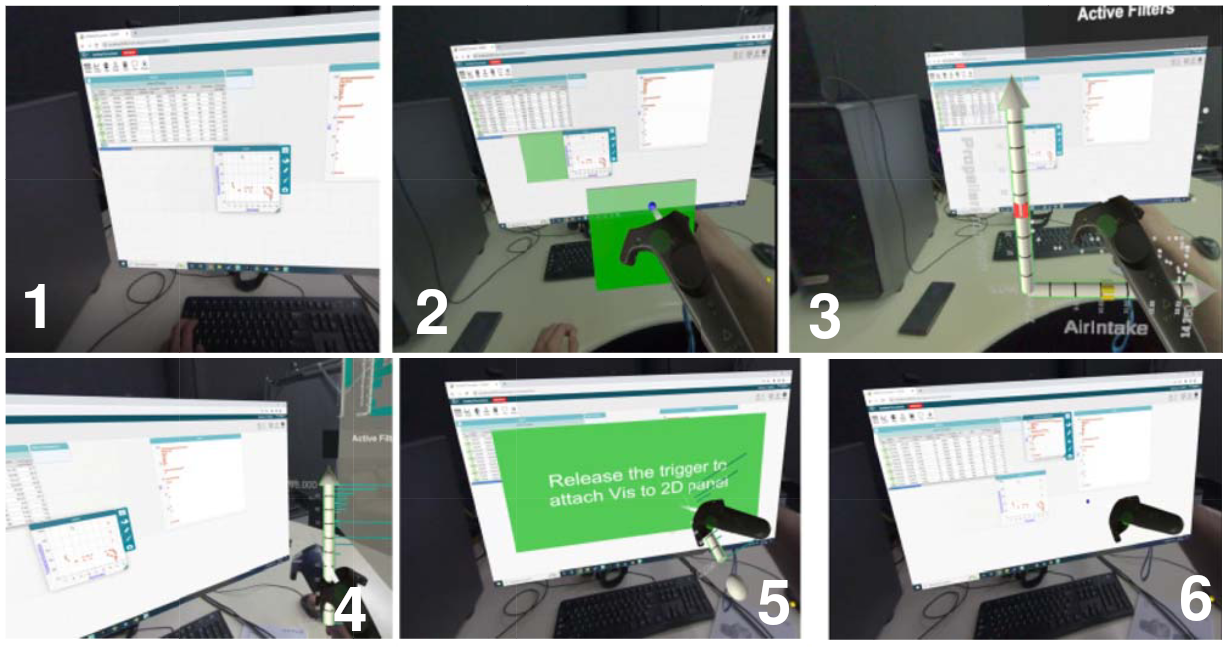
\includegraphics[width=\columnwidth]{hybridaxes}
	\caption[Caption for RagRug]{HybredAxes context switch processes. (1, 2, 3)
		Pulling data/visualization from a 2D screen. (4, 5, 6) Pushing a
		visualization to a 2D screen from an immersive AR environment.}
	\label{fig:hybridaxes}
\end{figure}

\noindent HybridAxes aims to provide a balanced feature set and performance
between the two ends of the Reality-Virtuality continuum while giving the users
the ultimate choice to choose which environment to work in. To avoid
disruptions of the user's flow when context switching, the tool also aims to
provide a smooth transition by reducing visualization generation delays. It
claims to do that by anticipating the user's interactions in both modes and
preemptively generating
visualizations in the background. Moreover, the authors stated that providing
a clear signaling of transition status either through visual (\cref{fig:hybridaxes} (2, 5)) or
controller-related feedback is a core design requirement for the tool.
Keeping the same values for the visualization channels, if possible, when
transitioning a visualization between the two experiences is also stated as
a core design goal. HybridAxes should also provide support for synchronized
cross-virtuality brushing and linking. For instance, a user may have a tabular
data on a 2D desktop alongside a 3D scatterplot in the immersive environment.
When highlighting an entry in the table, associated datapoints in the
scatterplot should also be highlighted. HybridAxes, aims to also favor desktop
for interactions that require the detailed manipulation of text entries. The
choice of interaction method, either through free-hand or
controller-based interactions, is given to the user.

\medskip

\noindent In terms of implementation, HybridAxes adopts CODAP; an open-source
\footnote{https://codap.concord.org} visual analytics tool, alongside a plugin
that enables the desktop system to receive commands via a Websocket interface.
A Node.js-based Websocket server is used to relay the messages between Unity
and the desktop system. We question the use of these extra tools and frameworks
since we believe that transitioning between immersive and 2D Unity
visualizations is superior to the suggested workflow. Our main argument is
that this way all visualizations are established within one framework - Unity -
which therefore allows for a more versatile, accessible and easier-to-use
toolkit. The tool provides support for the same set of visualizations as IATK
mainly: Scatterplots, Parrallel Coordinate Plots and Bar Charts.

\medskip

\noindent In terms of performance, the authors claim that anticipating user
actions has resulted in smoother experience. However, no comparative
performance measurements were provided to back this claim.

\smallskip

\noindent In terms of interactions, three types are supported:
\begin{itemize}
	\item \textbf{Pull visualizations from the 2D desktop} - by using free-hand gestures
	      or the controller(s) (\cref{fig:hybridaxes} (1, 2, 3)).
	\item \textbf{Push visualizations from the immersive environment back to the 2D
		      desktop} (\cref{fig:hybridaxes} (4, 5, 6)).
	\item \textbf{Brush datapoints on either side of the environments and see their
		      counterparts in the other side get highlighted}.
\end{itemize}


\noindent The authors hypothesize that enabling visual analytics users to
smoothly context switch between a 2D screen and 3D immersive experience could
improve their sensemaking abilities. A limited study of the usefulness of the
tool has been conducted on just four participants where they analyzed the data
in three scenarios: 1) just using 2D desktop screen, 2) using a hybrid
desktop/AR system and 3) just using the AR system. The authors claim that the
study results align with their hypothesis. However, neither metrics nor
sufficient details were provided to prove this claim. Nonetheless, the authors
mentioned their willingness to perform a more rigorous study in the future.

\section{Discussion}

Although the aforementioned toolkits and prototypes prove that the field of
immersive analytics is past its infancy stage, there are still many open
challenges with no proposed solutions yet.

\medskip

We believe that the following features and functionalities are yet to be
properly addressed altogether by the current state-of-art IA toolkits:

\begin{itemize}
	\item \textbf{Built on Open Standards} -
	\item \textbf{Permissive License} -
	\item \textbf{Visualization Tailored} - The toolkit should preferably be
	      built on top of a low-level extended reality library and be tailored
	      towards visualization tasks only.
	\item \textbf{Open Source} -
	\item \textbf{Uniform Workflow} - The toolkit should provide a unified
	      workflow to build IA experiences for a plethora of platforms.
	\item \textbf{Versatile Data Input Model} - The toolkit should make very
	      little assumptions about the format of the input data. In particular,
	      real-time data should be supported.
	\item \textbf{API with Bindings to High-level Programming Languages} - The
	      bindings should be good
\end{itemize}

Therefore we argue in favor of a visualization-tailored tool that is built on
top of open-standard XR technologies. We do particularly firmly believe that
an open-source and free-to-use - i.e. provides a permissive free software
license - tool built on top of the open-standard OpenXR API can mimic the
success of conventional 2D visualization libraries such as D3.js.
Unfortunately, we have not come across such a framework and the closest to that
in terms of reliance on open-standard technologies would be VRIA.

\section{Conclusion}
We presented an overview of the platforms, tools and prototypes in the last six
years which can be used to develop IA experiences. Although IA tools have
certainly come out of their infancy with several examples of tools addressing
particular IA challenges well, we have come to the conclusion that there is not
yet any IA toolkit that has the same level of versatility,
visualization-tailored, ease-of-use and support of various data inputs and
streams such as the widely successful 2D visualization libraries like D3.js.
This is consistent with the latest IA survey from 2021 \cite{survey_of_ia}
where no tool meeting these criteria was mentioned.

\printbibliography
\end{document}
